\section{Векторы}
\index{Векторы!компланарные} Векторы называются \textbf{компланарными}, если они лежат в одной плоскости, иначе~--- \textbf{некомпланарными}.

Некомпланарные векторы $\overline a, \overline b, \overline c$, начала которых находятся в одной точке, называются \textbf{правой тройкой~$(\overline a, \overline b, \overline c)$} (тройка имеет \textbf{правую ориентацию}), если с конца~$\overline c$ кратчайший поворот от~$\overline a$ к~$\overline b$ виден против часовой стрелки при условии, иначе~--- \textbf{левой тройкой~$(\overline a, \overline b, \overline c)$} (тройка имеет \textbf{левую ориентацию}).

Заметим, что тройки $(\overline a, \overline b, \overline c)$, $(\overline b, \overline c, \overline a)$, $(\overline c, \overline a, \overline b)$ всегда имеют одну ориентацию.

\subsection{Скалярное произведение}
\index{Произведение!скалярное} Пусть $\overline a = (x_1, y_1, z_1)$, $\overline b = (x_2, y_2, z_2)$.
Заметим, что $\overline i^2 = \overline j^2 = \overline k^2 = 1$, $\overline i\,\overline j = \overline i\,\overline k = \overline j\,\overline k = 0$.
Тогда
\begin{equation*}
\overline a\,\overline b =
(x_1 \overline i + y_1 \overline j + z_1 \overline k)(x_2 \overline i + y_2 \overline j + z_2 \overline k) =
x_1 x_2 + y_1 y_2 + z_1 z_2
\end{equation*}

\subsection{Векторное произведение}
\index{Произведение!векторное} \textbf{Векторным произведением векторов $\overline a$ и $\overline b$} называется вектор~$\overline c$ такой, что:
\begin{itemize}
	\item $|\overline c| = |\overline a| \cdot |\overline b| \cdot \sin \angle(\overline a, \overline b)$
	\item $\overline c \perp \overline a \lAnd \overline c \perp \overline b$
	\item $(\overline a, \overline b, \overline c)$~--- правая тройка
\end{itemize}
и обозначается $[\overline a \cdot \overline b]$ или $[\overline a\,\overline b]$.

По определению $|[\overline a\,\overline b]| = S$, где $S$~--- площадь параллелограмма, построенного на векторах $\overline a$ и $\overline b$.

\begin{statement}
$[\overline a\,\overline b] = \overline 0 \Leftrightarrow \overline a \parallel \overline b$.
\end{statement}
\begin{proof}
$[\overline a\,\overline b] = \overline 0 \Leftrightarrow
|\overline a| \cdot |\overline b| \cdot \sin \angle(\overline a, \overline b) = 0 \Leftrightarrow
|\overline a| = 0 \lOr |\overline b| = 0 \lOr \sin \angle(\overline a, \overline b) = 0 \Leftrightarrow
\overline a \parallel \overline b$.
\end{proof}

Свойства векторного произведения:
\begin{enumerate}
	\item $[\overline a\,\overline a] = \overline 0$
	\begin{proof}
	$\angle(\overline a, \overline a) = 0 \Rightarrow
	|[\overline a\,\overline a]| = |\overline a|^2 \cdot \sin \angle(\overline a, \overline a) = 0 \Rightarrow
	[\overline a\,\overline a] = \overline 0$.
	\end{proof}
	
	\item $[\overline a\,\overline b] = -[\overline b\,\overline a]$
	\begin{proof}
	Достаточно заметить, что тройки $(\overline a, \overline b, \overline c)$ и $(\overline b, \overline a, \overline c)$ имеют разную ориентацию.
	\end{proof}
	
	\item $\forall \alpha \in \mathbb R \ [(\alpha \overline a)\,\overline b] = \alpha [\overline a\,\overline b]$
	\begin{proof}
	\begin{enumerate}
		\item Пусть $\alpha < 0$, тогда $[(\alpha \overline a)\,\overline b] = -|\alpha| [\overline a\,\overline b] = \alpha [\overline a\,\overline b]$.
		\item Пусть $\alpha \geqslant 0$, тогда $[(\alpha \overline a)\,\overline b] = |\alpha| [\overline a\,\overline b] = \alpha [\overline a\,\overline b]$.
	\end{enumerate}
	\end{proof}
	
	\item $[(\overline a + \overline b)\,\overline c] = [\overline a\,\overline c] + [\overline b\,\overline c]$
	\begin{proof}
	\begin{enumerate}
		\item \begin{minipage}[t]{130mm}\noindent
		Пусть $\overline a, \overline b, \overline c$ лежат в плоскости~$\pi$, $[\overline a\,\overline c] \upuparrows [\overline b\,\overline c]$.
		Введём векторы $\overline e \colon \overline e \in \pi \lAnd \overline e \perp \overline c$ и $\overline g \colon \overline g \upuparrows [\overline a\,\overline c] \opbr\lAnd |\overline g| = 1$.
		
		Тогда
		\begin{equation*}
		[\overline a\,\overline c] = 
		|\overline a| \cdot |\overline c| \cdot \cos \angle(\overline a, \overline e) \cdot \overline g =
		|\pr_{\overline e} \overline a| \cdot |\overline c| \cdot \overline g
		\end{equation*}
		\begin{equation*}
		[\overline b\,\overline c] = 
		|\overline b| \cdot |\overline c| \cdot \cos \angle(\overline b, \overline e) \cdot \overline g =
		|\pr_{\overline e} \overline b| \cdot |\overline c| \cdot \overline g
		\end{equation*}
		\begin{equation*}
		[(\overline a + \overline b)\,\overline c] =
		|\pr_{\overline e} (\overline a + \overline b)| \cdot |\overline c| \cdot \overline g =
		|\pr_{\overline e} \overline a| \cdot |\overline c| \cdot \overline g +
		|\pr_{\overline e} \overline b| \cdot |\overline c| \cdot \overline g =
		[\overline a\,\overline c] + [\overline b\,\overline c]
		\end{equation*}
		
		Случай, когда $[\overline a\,\overline c] \updownarrows [\overline b\,\overline c]$, рассматривается аналогично.
		\end{minipage}
		\hfill
		\begin{minipage}[t]{33mm}\noindent
		\begin{flushright}
		\shorthandoff{"}
		\begin{tikzpicture}[>=latex]
		\def\angleC{20}
		\draw[->, name path=OC] (0, 0) coordinate (O) -- (\angleC:2.5) coordinate (C) node[above] {$\overline c$};
		\draw[->] (O) -- (-10:2) coordinate (A) node[below] {$\overline a$};
		\path[name path=AH] (A) -- +(\angleC + 90:2.5);
		\draw[name intersections={of=OC and AH, by=H}, dashed]
			(A) -- (H);
		
		\draw pic[draw, "$\varphi$", angle eccentricity=1.5, angle radius=7mm] {angle = A--O--C};
		
		\draw[->] (O) -- (\angleC + 90:-1) coordinate (E) node[left] {$\overline e$};
		\draw (O) -- (\angleC + 90:2)
			(E) -- (\angleC + 90:-2);
			
		\draw[->] (O) -- (0, 2) node[left] {$\overline g$};
		\end{tikzpicture}
		\shorthandon{"}
		\end{flushright}
		\end{minipage}
		
		\item Пусть $\overline a, \overline b, \overline c$ некомпланарны, тогда $[(\overline a + \overline b)\,\overline c], [\overline a\,\overline c], [\overline b\,\overline c] \perp \overline c \Rightarrow
		[(\overline a + \overline b)\,\overline c], [\overline a\,\overline c], [\overline b\,\overline c]$ компланарны $\Rightarrow$
		$\alpha [(\overline a + \overline b)\,\overline c] \opbr=
		\beta [\overline a\,\overline c] \opbr+ \gamma [\overline b\,\overline c]$.
		
		\begin{minipage}[t]{95mm}\noindent
		Докажем, что $\alpha = \beta$.
		\begin{itemize}
			\item $\alpha [(\overline a + \overline b)\,\overline c] =
			\beta [\overline a\,\overline c] + \gamma [\overline b\,\overline c] \Rightarrow
			\alpha (\overline a + \overline b)\,\overline c\,\overline b =
			\beta \overline a\,\overline c\,\overline b$
			
			\item Пусть $V_1$ и $V_2$~--- объёмы параллелепипедов, построенных на $OA$, $OB$, $OH$ и $OC$, $OB$, $OH$ соответственно, тогда $S(OACB) = S(OCDB) \opbr\Rightarrow
			V_1 = V_2 \opbr\Rightarrow
			\overline a\,\overline b\,\overline c = (\overline a + \overline b)\,\overline b\,\overline c \opbr\Rightarrow
			\overline a\,\overline c\,\overline b = (\overline a + \overline b)\,\overline c\,\overline b$
		\end{itemize}
		
		Отсюда $\alpha = \beta$.
		Аналогично $\alpha = \gamma$.
		\end{minipage}
		\hfill
		\begin{minipage}[t]{71mm}\noindent
		\begin{flushright}
		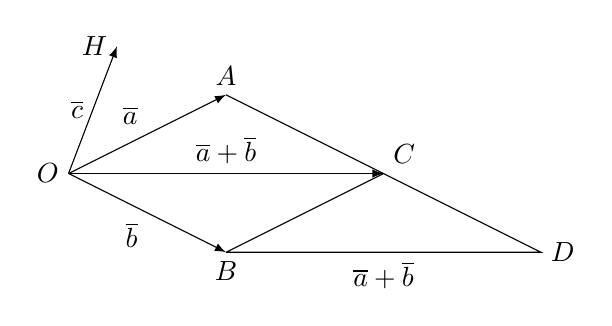
\begin{tikzpicture}[>=latex]
		\draw[->] (0, 0, 0) coordinate (O) node[left] {$O$}
				-- node[above left] {$\overline a$} (2, 1, 0) coordinate (A) node[above] {$A$};
		\draw[->] (O) -- node[below left] {$\overline b$} (2, -1, 0) coordinate (B) node[below] {$B$};
		\draw[->] (O) -- node[above] {$\overline a + \overline b$}
				(4, 0, 0) coordinate (C) node[above right] {$C$};
		\draw (C) -- (A)
			(B) -- (C) -- (6, -1, 0) coordinate (D) node[right] {$D$}
				-- node[below] {$\overline a + \overline b$} (B);
		\draw[->] (O) -- node[left] {$\overline c$} (1, 2, 1) coordinate (H) node[left] {$H$};
		\end{tikzpicture}
		\end{flushright}
		\end{minipage}
	\end{enumerate}
	\end{proof}
\end{enumerate}

Пусть $\overline a = (x_1, y_1, z_1)$, $\overline b = (x_2, y_2, z_2)$.
Заметим, что $[\overline i\,\overline i] = [\overline j\,\overline j] = [\overline k\,\overline k] = \overline 0$, $[\overline i\,\overline j] = \overline k$, $[\overline i\,\overline k] = -\overline j$, $[\overline j\,\overline k] = \overline i$.
Тогда
\begin{equation*}
[\overline a\,\overline b] =
[(x_1 \overline i + y_1 \overline j + z_1 \overline k)(x_2 \overline i + y_2 \overline j + z_2 \overline k)] =
\end{equation*}
\begin{equation*}
= (y_1 z_2 - y_2 z_1) \overline i - (x_1 z_2 - x_2 z_1) \overline j + (x_1 y_2 - x_2 y_1) \overline k =
\begin{vmatrix}
\overline i & \overline j & \overline k \\
x_1 & y_1 & z_1 \\
x_2 & y_2 & z_2
\end{vmatrix} =
\left(
\begin{vmatrix}
y_1 & z_1 \\
y_2 & z_2
\end{vmatrix},
-\begin{vmatrix}
x_1 & z_1 \\
x_2 & z_2
\end{vmatrix},
\begin{vmatrix}
x_1 & y_1 \\
x_2 & y_2
\end{vmatrix}
\right)
\end{equation*}

\subsection{Смешанное произведение}
\index{Произведение!смешанное} \textbf{Смешанным произведением векторов $\overline a$, $\overline b$ и $\overline c$} называется скалярное произведение вектора~$\overline c$ и векторного произведения~$[\overline a\,\overline b]$ и обозначается $[\overline a\,\overline b] \overline c$.

\begin{statement}
$[\overline a\,\overline b] \overline c = \pm V$, где $\pm V$~--- объём параллелепипеда, построенного на векторах $\overline a$, $\overline b$, $\overline c$, взятый со знаком плюс, если тройка $(\overline a, \overline b, \overline c)$ правая, или со знаком минус, если она левая.
\end{statement}

\noindent\begin{wrapfigure}{r}{0pt}\noindent
\shorthandoff{"}
\begin{tikzpicture}[scale=0.7]
% рисуем векторы и нижнюю часть параллелепипеда
\draw[->] (0, 0) coordinate (O) -- (3, 0) coordinate (A) node[below] {$\overline a$};
\draw[->] (O) -- (2, 3) coordinate (B) node[below right] {$\overline b$};
\draw[->] (O) -- (1, 3) coordinate (C) node[left] {$\overline c$};
\draw[->] (O) -- (0, 2) coordinate (G) node[left] {$\overline g$};
\draw (A) -- (5, 3) coordinate (D) -- (B);

% рисуем верхнюю часть параллелепипеда
\coordinate (prev) at (C);
\foreach \point in {O, A, D, B}
	\draw (\point) ++(C) coordinate (cur)
		(prev) -- (cur) coordinate (prev) -- (\point);
\draw (B) ++(C) -- (C);

% рисуем угол
\draw pic[draw, "$\psi$", angle eccentricity=1.5, angle radius=7mm] {angle = C--O--G};
\end{tikzpicture}
\shorthandon{"}
\end{wrapfigure}
\begin{proof}
Пусть $|[\overline a\,\overline b]| = S$, $\overline g \upuparrows [\overline a\,\overline b]$, $|\overline g| = 1$, тогда
\begin{equation*}
|[\overline a\,\overline b] \overline c| =
S(\overline g\,\overline c) =
S \cdot |\overline c| \cdot \cos \psi =
S \cdot (\pm h) = \pm V
\end{equation*}
где $h$~--- высота параллелепипеда.
\end{proof}

\begin{statement}
$[\overline a\,\overline b] \overline c = 0$ $\Leftrightarrow$ $\overline a, \overline b, \overline c$ компланарны.
\end{statement}
\begin{proof}
\begin{enumerate}
	\item $\Rightarrow$. Если $\overline a, \overline b, \overline c$ некомпланарны, то на них можно построить параллелепипед с ненулевым объёмом~$V$.
	Но $V = |[\overline a\,\overline b] \overline c| = 0$, значит, $\overline a, \overline b, \overline c$ компланарны.
	
	\item $\Leftarrow$. Можно считать, что $\overline a, \overline b, \overline c$ лежат в одной плоскости.
	Тогда $[\overline a\,\overline b] \perp \overline c \Rightarrow
	[\overline a\,\overline b] \overline c = 0$.
\end{enumerate}
\end{proof}

\begin{statement}
$[\overline a\,\overline b] \overline c = \overline a [\overline b\,\overline c]$.
\end{statement}
\begin{proof}
$\overline a [\overline b\,\overline c] = [\overline b\,\overline c] \overline a$.
Тройки $(\overline a, \overline b, \overline c)$ и $(\overline b, \overline c, \overline a)$ имеют одну ориентацию, тогда $[\overline b\,\overline c] \overline a = kV = \overline a [\overline b\,\overline c]$, где $V$~--- объём соответствующего параллелепипеда, $k = -1$, если эти тройки левые, или $k = 1$, если тройки правые.
\end{proof}

Т.\,о., вместо $[\overline a\,\overline b] \overline c$ допустима запись $\overline a\,\overline b\,\overline c$.

Пусть $\overline a = (x_1, y_1, z_1)$, $\overline b = (x_2, y_2, z_2)$, $\overline c = (x_3, y_3, z_3)$, тогда
\begin{equation*}
\overline a\,\overline b\,\overline c =
(y_1 z_2 - y_2 z_1) x_3 - (x_1 z_2 - x_2 z_1) y_3 + (x_1 y_2 - x_2 y_1) z_3 =
\begin{vmatrix}
x_1 & y_1 & z_1 \\
x_2 & y_2 & z_2 \\
x_3 & y_3 & z_3
\end{vmatrix}
\end{equation*}